\documentclass[a4paper,11pt,exos]{nsi} 
\usepackage{fontawesome5}

%\pagestyle{empty}


\begin{document}




\classe{\premiere Spé}
\titre{Corrigé de l'évaluation-bilan 6}
\maketitle



\exo{}
Lors du lancement d'un hebdomadaire (magazine publié chaque semaine), \np{1200} exemplaires ont été vendus.\\
Une étude de marché prévoit une progression des ventes de 2\,\% chaque semaine.\\
On modélise le nombre d'hebdomadaires vendus par une suite $\left(u_n\right)$ où $u_n$ représente le nombre de journaux vendus durant la $n$-ième semaine après le début de l'opération.\\
On a donc $u_0 = \np{1200}$.


\begin{enumerate}
\item Calculer le nombre $u_1$. Interpréter ce résultat dans le contexte de l'exercice.
\textcolor{UGLiBlue}{
    \begin{tabbing}
        $u_1$   \= $= 1200 \times 1,02$\\
        \> $= 1224$
    \end{tabbing}
    Donc le nombre d'hebdomadaires vendus durant la deuxième semaine est de 1224.
}
\item Préciser la nature de la suite $(u_n)$.\\
En déduire, pour tout entier naturel $n$, l'expression de $u_n$ en fonction de $n$.\\[.5em]
\textcolor{UGLiBlue}{
    La suite $(u_n)$ est une suite géométrique de premier terme $u_0 = 1200$ et de raison $q = 1,02$.
    \begin{tabbing}
        Donc, pour tout entier naturel $n$, on a : $\quad u_n$ \= $= u_0 \times q^n$\\
        \> $= 1200 \times 1,02^n$
    \end{tabbing}
}
\item Voici le programme complété pour que l'exécution de \mintinline{python}{semaine(30000)} renvoie le nombre de semaines nécessaires pour que le nombre total d'hebdomadaires vendus soit supérieur à \np{30000} :

\begin{pyc}
    \begin{minted}{python}
        def semaine(n) :
            u = 1200
            S = 1200
            n = 0
            while S < 30000 :
                n = n + 1
                u = 1.02 * u
                S = S + u
            return(n)
    \end{minted}
\end{pyc}
\item Déterminer par le calcul le nombre total d'hebdomadaires vendus au bout d'un an (52 semaines).\\[.5em]
\textcolor{UGLiBlue}{
    \begin{tabbing}
        $S_{51}$ \= $=u_0+u_1+u_2+\ldots+u_{51}$\\[.5em]
        \> $= u_0 \times \dfrac{1 - q^{52}}{1 - q}$\\[.5em]
        \> $= 1200 \times \dfrac{1 - 1,02^{52}}{1 - 1,02}$\\[.5em]
        \> $= 1200 \times \dfrac{1 - 1,02^{52}}{-0,02}$\\[.5em]
        \> $\approx 1200 \times 90,0164$\\
        \> $\approx \np{108020}$
    \end{tabbing}
    Donc le nombre total d'hebdomadaires vendus au bout d'un an est de 108 020.
}
\end{enumerate}


\exo{}
Une collectivité locale octroie une subvention de \np{166440} € pour le forage d'une nappe d'eau souterraine. \\
Une entreprise estime que le forage du premier mètre coûte 120 €; le forage du deuxième mètre coûte 60 € de plus que celui du premier mètre ; le forage du troisième mètre coûte 60 € de plus que celui du deuxième mètre, etc.\\
Plus généralement, le forage de chaque mètre supplémentaire coûte 60 € de plus que celui du mètre précédent.\\[.5em]    
Pour tout entier naturel $n$, on note: $u_n$ le coût (en euros) du forage après avoir creusé $n$ mètres et $T_n$ le coût (en euros) du forage de $n+1$ mètres ; ainsi $u_0=120$ et $T_0=120$.
    
\begin{enumerate}
    \item Calculer $u_1$ et $u_2$. Interpréter les résultats obtenus dans le contexte de l'exercice.
    \textcolor{UGLiBlue}{
        \begin{multicols}{2}
            \begin{tabbing}
                $u_1$ \= $=u_0+60$\\ 
                \>  $=120 + 60$\\
                \> $= 180$\\[.5em]
                $u_2$ \= $= u_1 + 60$\\
                \> $= 180 + 60$\\
                \> $= 240$
            \end{tabbing}
        \end{multicols}
        Donc le coût du forage du deuxième mètre est de 180 € et le coût du forage du troisième mètre est de 240 €.
    }
    \item Préciser la nature de la suite $\left(u_n\right)$\\
    En déduire l'expression de $u_n$ en fonction de $n$, pour tout entier naturel $n$.\\[.5em]
    \textcolor{UGLiBlue}{
        La suite $(u_n)$ est une suite arithmétique de premier terme $u_0 = 120$ et de raison $r = 60$.
        \begin{tabbing}
            Donc, pour tout entier naturel $n$, on a : $\quad u_n$ \= $= u_0 + n \times r$\\
            \> $= 120 + n \times 60$\\
            \> $= 120 + 60n$
        \end{tabbing}
    }
    \item  Pour tout entier naturel $n$, on note $T_n$ le coût total (en euros) du forage de $n+1$ mètres.\\
    Ainsi $T_0=120$ et $T_n=u_0+u_1+\ldots+u_n$.
    Calculer $T_1$ puis $T_2$. Interpréter les résultats obtenus dans le contexte de l'exercice.
    \textcolor{UGLiBlue}{
        \begin{multicols}{2}
            \begin{tabbing}
                $T_1$ \= $= u_0 + u_1$\\
                \> $= 120+180$\\
                \> $= 300$\\
                $T_2$ \= $= u_0 + u_1 + u_2$\\
                \> $= 120 + 180 + 240$\\
                \> $= 540$
            \end{tabbing}
        \end{multicols}
        Donc le coût total du forage de 2 mètres est de 300 € et le coût total du forage de 3 mètres est de 540 €.
    }
    \item \begin{enumalph}
        \item Démontrer que, pour tout entier naturel $n$, $T_n = 30n^2+150n+120$.
        \textcolor{UGLiBlue}{
            \begin{tabbing}
                $T_n$ \= $= u_0 + u_1 + u_2 + \ldots + u_n$\\[.5em]
                \> $= (n+1) \times \dfrac{u_0 + u_n}{2}$\\[.5em]
                \> $= (n+1) \times \dfrac{120 + (120 + 60n)}{2}$\\[.5em]
                \> $= (n+1) \times \dfrac{120 + 120 + 60n}{2}$\\[.5em]
                \> $= (n+1) \times \dfrac{240 + 60n}{2}$\\[.5em]
                \> $= (n+1) (120 + 30n)$\\
                \> $= 120n + 120 + 30n^2 + 30n$\\
                \> $= 30n^2 + 150n + 120$
            \end{tabbing}
        }
        \item En déduire par le calcul la longueur maximale que l'entreprise peut forer avec la subvention de 166 440 €.
        \textcolor{UGLiBlue}{
            \begin{tabbing}
                $T_n\leqslant \np{166440}\quad$\= $\iff \quad 30n^2 + 150n + 120 \leqslant \np{166440}$\\
                \> $\iff \quad 30n^2 + 150n - \np{166320} \leqslant 0$
            \end{tabbing}
            Calcul du discriminant :
            \begin{tabbing}
                $\Delta$ \= $= 150^2 - 4 \times 30 \times (-\np{166320})$\\
                \> $= \np{22500} + \np{19958400}$\\
                \> $= \np{19980900}$
            \end{tabbing}
            Calcul des racines :
            \begin{tabbing}
                $n_1$ \= $= \dfrac{-150 - \sqrt{19980900}}{2 \times 30}$\\[.5em]
                    \> $= \dfrac{-150 - 4470}{60}$\\[.5em]
                    \> $= \dfrac{-4620}{60}$\\[.5em]
                    \> $= -77$\\[.5em]
                $n_2$ \= $= \dfrac{-150 + \sqrt{19980900}}{2 \times 30}$\\[.5em]
                    \> $= \dfrac{-150 + 4470}{60}$\\[.5em]
                    \> $= \dfrac{4320}{60}$\\[.5em]
                    \> $= 72$
            \end{tabbing}
            On a donc le tableau de signes suivant :
            \begin{center}
                \begin{tikzpicture}
                \tkzTabInit[color,lgt=7,espcl=2]
                {$n$/.7,Signe de $30n^2+150n-166\ 320$ /1}
                {$-\infty$,$-77$,$72$, $+\infty$}
                \tkzTabLine{,+,z,-,z,+,}
                \end{tikzpicture}
                \end{center}
            Donc la longueur maximale que l'entreprise peut forer avec la subvention de 116 610 € est de 73 mètres.}
    \end{enumalph}
    
    \end{enumerate}


\end{document}